\section{Technical appendix}

This appendix gives the estimator algebra, proofs, legacy optimization geometry, and the
equation-to-code map. The empirical tables and two detailed validation figures follow the
mathematical material.

\subsection{Joint covariance estimator}\label{app:covariance_proof}

Let \(F\in\R^{T\times k}\) and \(R\in\R^{T\times n}\) be centered, date-aligned factor and
option-return matrices. The decision-date Greek matrix is \(B^G\in\R^{n\times k}\). The
residual matrix is not an OLS residual matrix:
\begin{equation}
  E=R-F(B^G)^\top.
  \label{eq:app_residuals}
\end{equation}
Because \(B^G\) comes from marks and Greeks, no normal equation sets \(F^\top E\) to zero.
The cross covariance \(\widehat\Gamma=F^\top E/(T-1)\) is therefore estimated and retained.

Set \(Z=[F\ E]\) and let \(D=\diag(s_1,\ldots,s_{k+n})\) contain its sample standard
deviations. A zero-scale column uses a safe unit divisor during standardization and
returns to zero when rescaled. With \(\widetilde Z=ZD^{-1}\), the standardized
Ledoit-Wolf estimate has the form
\begin{equation}
  \widehat S_{LW}=(1-\widehat\rho)
  \frac{\widetilde Z^\top\widetilde Z}{T}
  +\widehat\rho\,\widehat\tau I.
  \label{eq:app_lw}
\end{equation}
The implementation uses the finite-sample shrinkage coefficient returned by the standard
Ledoit-Wolf estimator, then rescales:
\begin{equation}
  \widehat S_Z=D\widehat S_{LW}D
  =\begin{bmatrix}
    \widehat\Omega&\widehat\Gamma\\
    \widehat\Gamma^\top&\widehat\Sigma_\varepsilon
  \end{bmatrix}.
  \label{eq:app_rescaled_joint}
\end{equation}
Congruence by \(D\) preserves positive semidefiniteness. A second congruence by
\(H=[B^G\ I]\) gives \(\widetilde\Sigma_O=H\widehat S_ZH^\top\succeq0\). Floating-point
asymmetry is removed before the eigendecomposition
\begin{equation}
  \widehat\Sigma_O=Q\diag\{\max(\xi_j,10^{-10})\}Q^\top,
  \qquad
  \frac{\widetilde\Sigma_O+\widetilde\Sigma_O^\top}{2}
  =Q\diag(\xi_j)Q^\top.
  \label{eq:app_eigen_floor}
\end{equation}
This final operation is a numerical floor, not another statistical shrinkage model.

The unregularized identity is useful for testing. If
\(\widehat S_Z=Z^\top Z/(T-1)\), then
\begin{align}
  H\widehat S_ZH^\top
  &=\frac{1}{T-1}(ZH^\top)^\top(ZH^\top) \nonumber\\
  &=\frac{1}{T-1}\{F(B^G)^\top+E\}^\top
    \{F(B^G)^\top+E\}
   =\frac{R^\top R}{T-1}.
  \label{eq:app_sample_reconstruction}
\end{align}
Thus both cross terms are necessary for exact reconstruction. Setting
\(\widehat\Gamma=0\) would describe a different estimator.

\subsection{Breadth and mean error}\label{app:mean_error_proof}

Let \(e_i=\widehat\mu_i-\mu_i\), and suppose
\(\E[\exp(se_i)]\le\exp(s^2\bar\sigma^2/(2T))\) for every \(i\). Applying the same bound
to \(-e_i\) gives, for \(s>0\),
\begin{align}
  \E\left[\max_i|e_i|\right]
  &\le\frac{1}{s}\log\E\left[\sum_{i=1}^n
       \{e^{se_i}+e^{-se_i}\}\right] \nonumber\\
  &\le\frac{\log(2n)}{s}+\frac{s\bar\sigma^2}{2T}.
  \label{eq:app_max_bound}
\end{align}
Minimizing the right side at
\(s=\sqrt{2T\log(2n)}/\bar\sigma\) proves
Equation~\eqref{eq:max_mean_error}.

For any \(\|w\|_1\le g\), Holder's inequality gives
\begin{equation}
  |e^\top w|\le\|e\|_\infty\|w\|_1\le g\|e\|_\infty.
  \label{eq:app_objective_error}
\end{equation}
Let \(w^*\) maximize the true cost-aware utility and \(\widehat w\) maximize the same
utility with \(\widehat\mu\). Adding and subtracting estimated utility, then using the two
optimality inequalities, yields
\begin{equation}
  J_\mu(w^*)-J_\mu(\widehat w)
  \le2g\|\widehat\mu-\mu\|_\infty.
  \label{eq:app_regret}
\end{equation}
If a structural estimator has uniform bias at most \(\beta\), the raw cross-sectional
mean bound is smaller only while
\begin{equation}
  n<\frac12\exp\!\left(\frac{T\beta^2}{2\bar\sigma^2}\right).
  \label{eq:app_crossover}
\end{equation}
Beyond this crossover, the stated structural bias bound is smaller than the stated raw
mean bound. The comparison does not rank the estimators by total error because it does
not bound the structural estimator's variance. It only shows how the raw mean bound
changes when contract breadth rises without a longer training sample.

\subsection{Optimality conditions and shadow prices}\label{app:kkt_proof}

Write every feasible-set inequality as \(g_j(w,\eta)\le0\), including the sample-CVaR
epigraph, and retain linear equalities as \(h_l(w)=0\). The convex minimization form of
Equation~\eqref{eq:net_utility} has Lagrangian
\begin{equation}
  \mathcal L(w,\eta,\rho,\zeta)
  =-\widehat\mu^\top w+\kappa(w)
   +\frac{\lambda}{2}w^\top\Sigma_Ow
   +\sum_j\rho_jg_j(w,\eta)+\sum_l\zeta_lh_l(w),
  \label{eq:app_lagrangian}
\end{equation}
where \(\rho_j\ge0\). Under the usual relative-interior qualification, the KKT system is
\begin{align}
  0&\in-\widehat\mu+\partial\kappa(w^*)+\lambda\Sigma_Ow^*
       +\sum_j\rho_j^*\partial_w g_j(w^*,\eta^*)
       +\sum_l\zeta_l^*\nabla h_l(w^*), \label{eq:app_kkt_w}\\
  0&\in\sum_j\rho_j^*\partial_\eta g_j(w^*,\eta^*), \label{eq:app_kkt_eta}\\
  g_j(w^*,\eta^*)&\le0,\qquad h_l(w^*)=0,\qquad \rho_j^*\ge0, \nonumber\\
  \rho_j^*g_j(w^*,\eta^*)&=0. \label{eq:app_kkt_comp}
\end{align}
These conditions are sufficient because the problem is convex. They reduce to
Equation~\eqref{eq:kkt_subgradient} when the individual constraint normals are collected
in \(N_{\mathcal C}(w^*)\).

The multiplier on a binding right-hand-side budget measures the local gain in optimized
utility from relaxing that budget, subject to the regularity conditions for sensitivity
analysis. A high CVaR multiplier identifies scarce tail capacity. The same reading applies
to stress, liquidity, margin, collateral, beta, and vega multipliers. Zero multipliers on
slack limits prevent a post hoc story in which every listed constraint is said to drive
the portfolio.

For completeness, the sample-CVaR term can be written without positive-part notation.
Introduce \(u_k\ge0\) and impose
\begin{equation}
  u_k\ge L_k(w)-\eta\quad(k=1,\ldots,K),
  \qquad
  \eta+\frac{1}{(1-\alpha)K}\sum_{k=1}^K u_k\le L^{CVaR}.
  \label{eq:app_cvar_linearization}
\end{equation}
For fixed \((w,\eta)\), minimizing the left side sets
\(u_k=[L_k(w)-\eta]_+\). The auxiliary formulation is therefore equivalent to
Equation~\eqref{eq:cvar_epigraph}. Since \(L_k(w)\) is convex after asymmetric costs,
these epigraph inequalities remain convex. The solver handles them together with the
quadratic risk term through its conic interface.

\subsection{Finite scale and conservative changes}

\begin{lemma}[No free option scale]
For any nonzero premium-weight direction \(d\), the feasible ray
\(\{ad:a\ge0\}\cap\mathcal C\) is bounded.
\end{lemma}
\begin{proof}
The gross-premium constraint requires \(a\|d\|_1\le1\). Since \(d\ne0\),
\(a\le1/\|d\|_1<\infty\). A direction with \(d=0\) has no option premium, payoff, or
Greek exposure and is economically empty. The additional stress, margin, assignment, and
liquidity limits can only shorten the feasible ray.
\end{proof}

Define \(V(\mathcal C,c_+,c_-)\) as the optimized value of
Equation~\eqref{eq:net_utility}. If \(\mathcal C_1\subseteq\mathcal C_0\),
\(c_{+,1}\ge c_{+,0}\), and \(c_{-,1}\ge c_{-,0}\) componentwise, then
\begin{equation}
  V(\mathcal C_1,c_{+,1},c_{-,1})
  \le V(\mathcal C_0,c_{+,0},c_{-,0}).
  \label{eq:app_conservative_value}
\end{equation}
Every point feasible under the tighter rules was feasible before, and its new cost is no
smaller. This ordering concerns optimized utility, not realized return. It is the correct
formal statement behind the spread and capacity sensitivity checks.

\subsection{Legacy maximum-Sharpe reduction}

The legacy E1 specification used a ratio objective that is not the accepted R1 or R1.1
program.
For \(\Sigma\succ0\), excess-mean vector \(a\), and convex cone \(K\), consider
\begin{equation}
  \max_{w\in K\setminus\{0\}}
  \frac{a^\top w}{\sqrt{w^\top\Sigma w}}.
  \label{eq:app_sharpe_ratio}
\end{equation}
The ratio is homogeneous of degree zero. Any direction with positive numerator can be
normalized to variance one, which gives the conic problem
\begin{equation}
  \max_{y\in K}\ a^\top y
  \quad\text{subject to}\quad
  \|\Sigma^{1/2}y\|_2\le1.
  \label{eq:app_sharpe_socp}
\end{equation}
Conversely, any nonzero optimizer of Equation~\eqref{eq:app_sharpe_socp} supplies an
optimal ratio direction. Without constraints, that direction is proportional to
\(\Sigma^{-1}a\).

This reduction does not choose an economically valid option scale. It also does not
represent the asymmetric piecewise-linear costs, admissible cash, sample CVaR, or
whole-contract acceptance rule in Equation~\eqref{eq:net_utility}. E1 used it for
selection; R1 and R1.1 do not.

\subsection{R1.1 geometry and integer acceptance}

\begin{proposition}[Convex sign-restricted augmentation]
After the first-stage signs \(s\) are fixed, the feasible set in
Equation~\eqref{eq:r11_feasibility} is convex, and gross premium is \(\one^\top x\).
Therefore the maximum-feasible-gross problem and the conditional 50 percent utility
problem have global solutions whenever they are feasible.
\end{proposition}
\begin{proof}
The map \(x\mapsto s\odot x\) is linear. The inverse image of \(\mathcal C_t\) under this
map is convex. Nonnegativity, eligibility, total edge, and gross limits are linear. The
variance cap is a convex quadratic inequality because \(\Sigma_O\succeq0\). Finally,
\(|s_i x_i|=x_i\) on every retained nonzero sign, so
\(\|s\odot x\|_1=\one^\top x\). Both objectives are concave or linear on this set.
\end{proof}

The feasibility stage matters because an equality such as \(\one^\top x=0.50\) can make
an otherwise valid convex program infeasible. Solving for \(G^*\) first distinguishes an
economic target from an available risk and liquidity budget. In the historical replay,
\(G^*<0.50\) at every decision, so the equality branch was never entered.

Truncating each contract count toward zero reduces the premium magnitude of every leg,
but it does not prove portfolio feasibility. A smaller hedge can increase net beta, vega,
or scenario loss because those constraints depend on signed sums. The direct book must
therefore pass the same diagnostic function as the continuous target. This is also why
the policy does not drop a negative standalone-edge hedge during integer conversion. The
accepted action is the exact truncation when feasible and cash otherwise.

The size of the discretization error is explicit. Let
\(u_i=100C_i/W\) be one contract expressed as a NAV weight and let
\(\delta=\widehat w-w\). Truncation on a fixed sign gives
\begin{equation}
  |\delta_i|<u_i\quad\text{for every active leg},
  \qquad
  \|\delta\|_1<\sum_{i\in\mathcal I(w)}u_i.
  \label{eq:app_integer_error}
\end{equation}
Consequently,
\begin{align}
  |\widehat\mu^\top\delta|
  &\le\|\widehat\mu\|_\infty\|\delta\|_1, \\
  |\kappa(\widehat w)-\kappa(w)|
  &\le\max_i(c_{+,i},c_{-,i})\|\delta\|_1, \\
  |\widehat w^\top\Sigma_O\widehat w-w^\top\Sigma_Ow|
  &\le\|\Sigma_O\|_2\|\delta\|_2
       (\|\widehat w\|_2+\|w\|_2).
  \label{eq:app_integer_risk_error}
\end{align}
These bounds shrink with account NAV and grow with option price. They measure
discretization error, but signed exposure cancellations can still change after
truncation. Exact constraint rechecking remains necessary.

\subsection{Purging and path construction}

\begin{lemma}[Holding-window purge]
Suppose label \(j\) uses information from a holding interval \([t_j,t_j+h_j]\). Removing
every training label whose interval intersects a test interval prevents a realized return
used in a test label from also entering a training label.
\end{lemma}
\begin{proof}
If one realized return entered both labels, its date would belong to both holding
intervals, so the intervals would intersect. The purge rule would have removed that
training label, a contradiction.
\end{proof}

The implementation also embargoes observations adjacent to each test block and checks the
realized calendar gap on both sides. Purging prevents label-window overlap; it does not
assert statistical independence of nonoverlapping market returns. Recombined CPCV paths
retain time order within each test block. Wealth stays at zero after any return of
\(-100\) percent or less, so later arithmetic ratios cannot revive an absorbed path.

\clearpage
\subsection{Equation-to-code map}\label{app:code_map}

The public package implements the pricing, covariance, allocation, policy, and inference
objects used in the paper. Historical factor construction and conditional-mean estimation
depended on licensed feature stores. Those stages are represented by source hashes and
derived evidence, not by a public regeneration pipeline.

\begingroup
\small
\setlength{\tabcolsep}{4pt}
\noindent
\begin{tabularx}{\textwidth}{@{}L{0.16\textwidth} L{0.28\textwidth} >{\raggedright\arraybackslash}X@{}}
\toprule
Object & Public implementation or boundary & Role \\
\midrule
Pricing and Greek loadings
& \path{bs_price}, \path{bs_greeks},
  \path{greek_exposure_frame}, \path{risk_exposure_frame}
& Prices the option and constructs the factor and policy-risk loadings. \\
Joint covariance
& \path{estimate_greek_joint_moments}
& Estimates Equations~\eqref{eq:app_residuals}-\eqref{eq:app_rescaled_joint}; the model
  constructor applies Equation~\eqref{eq:complete_covariance} and the eigenvalue floor. \\
Historical factors and means
& Recorded source hashes and derived evidence
& The public model accepts prepared expected returns and joint moments; it does not
  reconstruct the licensed feature stores behind
  Equations~\eqref{eq:structural_mean}-\eqref{eq:mean_shrinkage}. \\
Costs and assignment inputs
& \path{OptimizationCostSpec}
& Validates prepared \(c_+\), \(c_-\), short-margin coefficients, and admissible-short
  flags. \\
R1 constraints
& \path{r1_constraints}, \path{_net_utility_constraints}
& Constructs and applies Equations~\eqref{eq:basic_limits}-\eqref{eq:cvar_epigraph}. \\
R1 objective and risk search
& \path{solve_net_utility}
& Solves Equation~\eqref{eq:net_utility} and performs the 18-step log bisection. \\
Independent diagnostics
& \path{validate_portfolio}
& Recomputes tail, stress, funding, assignment, and liquidity breaches. \\
R1.1 augmentation
& \path{solve_r11_net_utility}
& Implements Equations~\eqref{eq:r11_directions}-\eqref{eq:r11_feasibility}. \\
Whole-contract acceptance
& \path{integerize_or_cash}
& Applies Equation~\eqref{eq:integer_conversion}, rechecks the book, and selects direct
  execution or cash. \\
Inference
& \path{probabilistic_sharpe_ratio}, \path{deflated_sharpe_ratio}
& Computes the finite-sample Sharpe statistics reported with the retained evidence. \\
\bottomrule
\end{tabularx}
\endgroup

\FloatBarrier
\subsection{Licensed-quote audit tables}\label{app:audit_tables}

Table~\ref{tab:app_execution_summary} contains the complete scenario ladder. The audit
aggregates coverage by absolute portfolio weight. Missing quote legs retain modeled spread
cost, and the coverage denominator still counts them.
Table~\ref{tab:app_spread_sources} records the source mix, while
Tables~\ref{tab:app_execution_spreads} and~\ref{tab:app_liquidity} report the spread and
entry-date liquidity checks.

\begin{table}[H]
\centering
\caption{Historical spread-source ladder by universe. The counts describe cost-evidence
rows, not orders or realized executions.}
\label{tab:app_spread_sources}
\begin{tabular}{lrrrr}
\toprule
Configuration & Exact CBBO rows & Proxy rows & Proxy share & Median spread \\
\midrule
orig & 5777 & 0 & 0.000 & 0.019 \\
orig+VIX & 5777 & 536 & 0.085 & 0.022 \\
larger & 5777 & 23740 & 0.804 & 0.019 \\
larger+VIX & 5777 & 24276 & 0.808 & 0.020 \\
\bottomrule
\end{tabular}

\end{table}

\begin{table}[H]
\centering
\caption{R1.1 CAGR, Sortino ratio, drawdown, and quote coverage under the modeled,
midpoint, touch-price, and worst-quote scenarios.}
\label{tab:app_execution_summary}
\small
\begin{tabular}{llrrrrr}
\toprule
Book & Cost scenario & CAGR & Sortino & MaxDD & Entry \% & Round trip \% \\
\midrule
larger & modeled & 0.123 & 1.114 & -0.394 & 98.472 & 62.902 \\
larger & midpoint & 0.130 & 1.176 & -0.391 & 98.472 & 62.902 \\
larger & touch price & 0.066 & 0.664 & -0.413 & 98.472 & 62.902 \\
larger & worst quote & 0.057 & 0.590 & -0.418 & 98.472 & 62.902 \\
\addlinespace
larger+VIX & modeled & 0.142 & 2.197 & -0.121 & 96.157 & 29.134 \\
larger+VIX & midpoint & 0.145 & 2.254 & -0.121 & 96.157 & 29.134 \\
larger+VIX & touch price & 0.121 & 1.812 & -0.128 & 96.157 & 29.134 \\
larger+VIX & worst quote & 0.119 & 1.771 & -0.129 & 96.157 & 29.134 \\
\addlinespace
orig & modeled & 0.118 & 1.097 & -0.381 & 98.696 & 65.061 \\
orig & midpoint & 0.123 & 1.145 & -0.378 & 98.696 & 65.061 \\
orig & touch price & 0.086 & 0.830 & -0.389 & 98.696 & 65.061 \\
orig & worst quote & 0.080 & 0.784 & -0.390 & 98.696 & 65.061 \\
\addlinespace
orig+VIX & modeled & 0.160 & 2.275 & -0.171 & 94.096 & 25.504 \\
orig+VIX & midpoint & 0.163 & 2.322 & -0.167 & 94.096 & 25.504 \\
orig+VIX & touch price & 0.146 & 2.052 & -0.185 & 94.096 & 25.504 \\
orig+VIX & worst quote & 0.145 & 2.029 & -0.186 & 94.096 & 25.504 \\
\bottomrule
\end{tabular}

\end{table}

\begin{table}[H]
\centering
\caption{Modeled and observed relative-spread quantiles by policy and quote regime.}
\label{tab:app_execution_spreads}
\resizebox{0.92\textwidth}{!}{\begin{tabular}{lrrrrrr}
\toprule
Arm & Regime & Source & p25 & p50 & p75 & p90 \\
\midrule
R1 & post\_2023\_03\_28 & modeled & 0.012 & 0.015 & 0.017 & 0.030 \\
R1 & post\_2023\_03\_28 & observed & 0.028 & 0.046 & 0.078 & 0.133 \\
R1 & pre\_2023\_03\_28 & modeled & 0.011 & 0.016 & 0.017 & 0.034 \\
R1 & pre\_2023\_03\_28 & observed & 0.013 & 0.026 & 0.049 & 0.081 \\
R1.1 & post\_2023\_03\_28 & modeled & 0.011 & 0.015 & 0.016 & 0.024 \\
R1.1 & post\_2023\_03\_28 & observed & 0.026 & 0.044 & 0.073 & 0.124 \\
R1.1 & pre\_2023\_03\_28 & modeled & 0.013 & 0.017 & 0.018 & 0.027 \\
R1.1 & pre\_2023\_03\_28 & observed & 0.014 & 0.024 & 0.042 & 0.071 \\
\bottomrule
\end{tabular}
}
\end{table}

\begin{table}[H]
\centering
\caption{Median entry-date participation and threshold breaches in the licensed-quote
audit.}
\label{tab:app_liquidity}
\small
\begin{tabular}{lrrrrrr}
\toprule
Policy & Vol. sum p50 & Vol. max p50 & OI p50 & Opt. fail & Vol. fail & OI fail \\
\midrule
R1 & 0.002 & 0.006 & 0.000 & 83 & 27 & 54 \\
R1.1 & 0.004 & 0.011 & 0.001 & 186 & 57 & 140 \\
\bottomrule
\end{tabular}

\end{table}

\FloatBarrier
\subsection{Integer, concentration, and validation tables}

The integer ledger in Table~\ref{tab:app_integer} reports accepted books and cash outcomes
separately. Tables~\ref{tab:app_concentration} and~\ref{tab:app_cpcv} retain E1
concentration and validation evidence.

\begin{table}[t]
\centering
\caption{Whole-contract direct conversion and cash outcomes for R1.1 base and diagnostic
books.}
\label{tab:app_integer}
\resizebox{0.74\textwidth}{!}{\begin{tabular}{lrrr}
\toprule
Method & Candidates & Feasible & Selected \\
\midrule
Cash abstention & 744 & 744 & 123 \\
Direct truncation & 744 & 621 & 621 \\
\bottomrule
\end{tabular}
}
\end{table}

\begin{table}[t]
\centering
\caption{E1 contract breadth, concentration, deployed gross, and capacity budget
at the stated account size.}
\label{tab:app_concentration}
\resizebox{0.88\textwidth}{!}{\begin{tabular}{lrrrrrr}
\toprule
Config & Candidates & Active & Top 5 share & Deployed gross & At cap share & Cap budget \\
\midrule
orig & 49 & 47 & 0.421 & 0.497 & 0.064 & 0.739 \\
orig+VIX & 54 & 54 & 0.324 & 0.723 & 0.093 & 1.093 \\
larger & 262 & 243 & 0.233 & 0.594 & 0.078 & 1.160 \\
larger+VIX & 267 & 253 & 0.296 & 0.836 & 0.083 & 1.515 \\
\bottomrule
\end{tabular}
}
\end{table}

\begin{table}[t]
\centering
\caption{E1 CPCV Sharpe quantiles, default shares, and relative-path evidence for the
liquid and claim windows. Liquid-window Sharpe is NA for configurations whose paths
reach zero wealth.}
\label{tab:app_cpcv}
\resizebox{\textwidth}{!}{\begin{tabular}{lrrrrrrr}
\toprule
Config & Liquid SR p05 & Liquid SR p50 & Default share & Claim SR p05 & Claim SR p50 & Rel. liquid p05 & Rel. claim p05 \\
\midrule
orig & 0.860 & 0.908 & 0.000 & 0.437 & 0.490 & -0.561 & -0.125 \\
orig+VIX & NA & NA & 1.000 & 1.003 & 1.062 & 0.214 & 2.257 \\
larger & 0.766 & 0.802 & 0.000 & 0.660 & 0.706 & -0.265 & -0.152 \\
larger+VIX & NA & NA & 1.000 & 1.445 & 1.474 & 0.103 & 1.501 \\
\bottomrule
\end{tabular}
}
\end{table}

\FloatBarrier
\subsection{Relocated path figures}

Figures~\ref{fig:app_walk_forward} and~\ref{fig:app_validation_distributions} retain the
detailed path and distribution views used by the verification suite.

\begin{figure}[!ht]
\centering
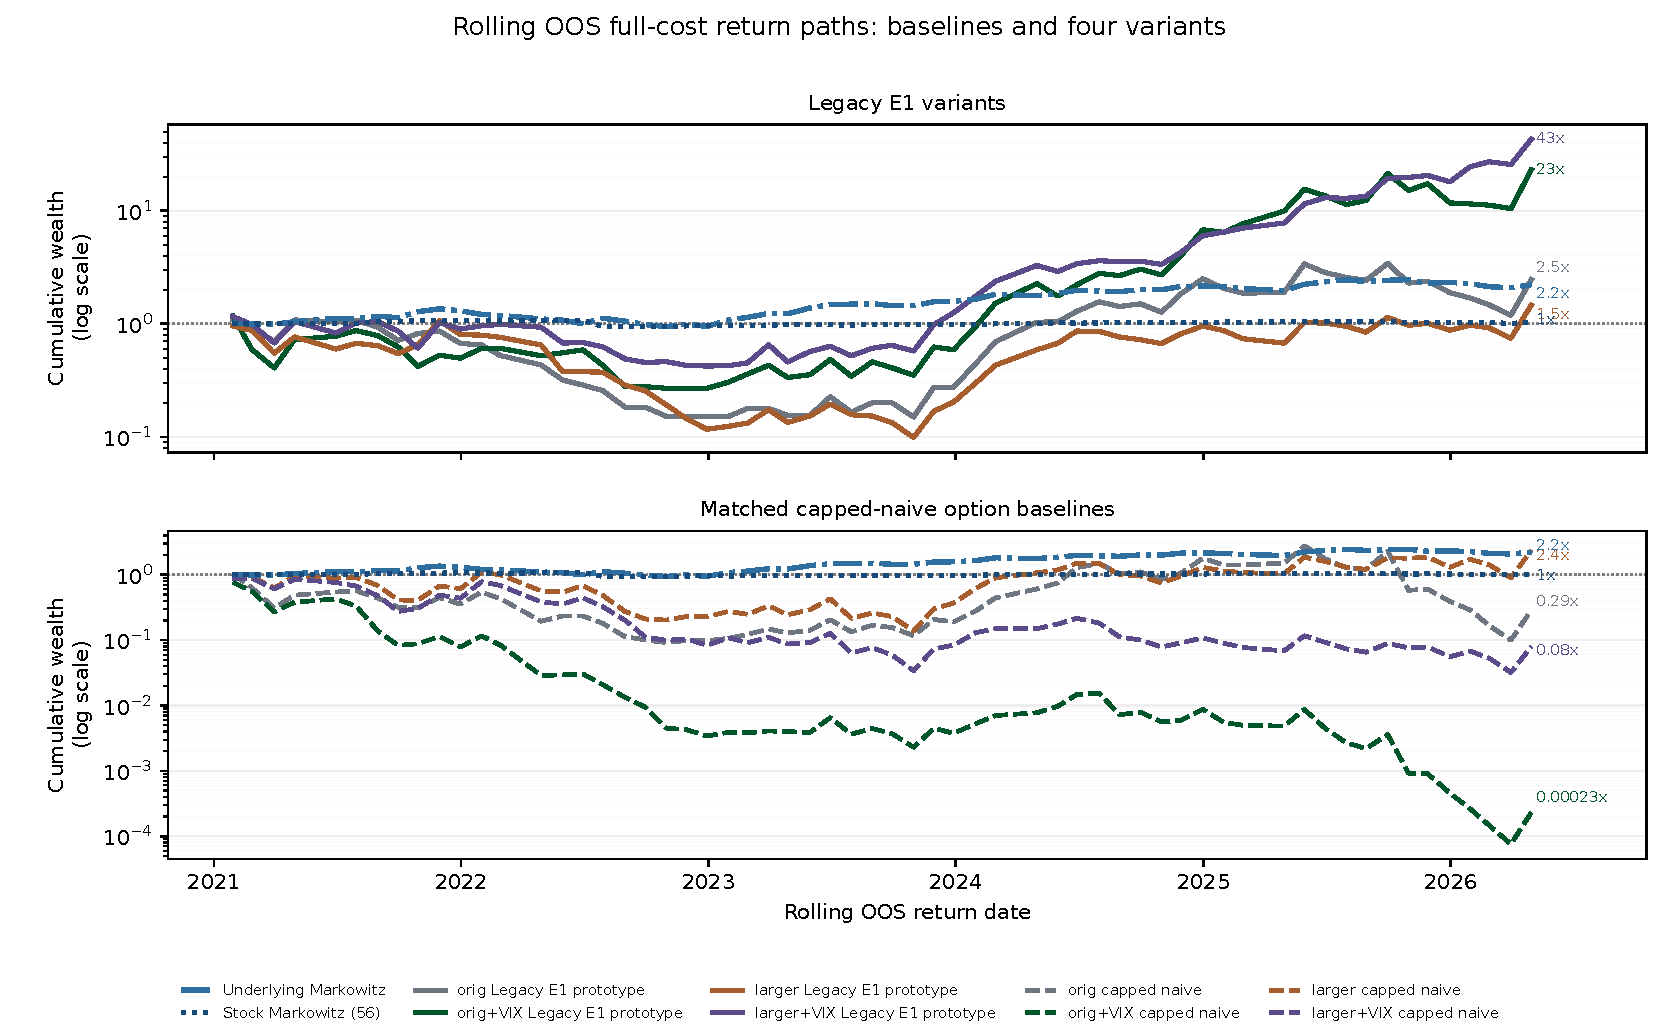
\includegraphics[width=0.94\textwidth]{figures/short_walk_forward_return_paths.pdf}
\caption{Rolling out-of-sample full-cost return paths for stock baselines, E1 universes,
and capped naive option books.}
\label{fig:app_walk_forward}
\end{figure}

\begin{figure}[!ht]
\centering
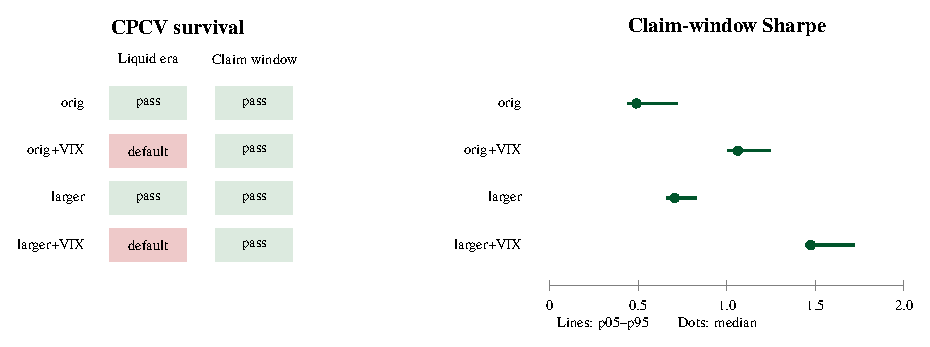
\includegraphics[width=0.93\textwidth]{figures/short_validation_distributions.pdf}
\caption{CPCV validation for the four E1 universes. The left panel reports survival in
the liquid and claim windows. The right panel shows claim-window Sharpe quantiles; no
Sharpe result is reported for a liquid-window path that defaults.}
\label{fig:app_validation_distributions}
\end{figure}

\FloatBarrier
